
% !TeX spellcheck = de_DE

\documentclass{article}

\usepackage[ngerman]{babel}
\usepackage{graphicx}
\usepackage{indentfirst}
\usepackage{hyperref}
\usepackage{geometry}
\usepackage{changepage}
\usepackage{booktabs}
\usepackage{float}
\usepackage{tabulary}
\usepackage{xcolor}
\usepackage{multirow}
\usepackage{caption}
\usepackage{subcaption}
\usepackage{lscape}
\usepackage{colortbl}
\usepackage{listings}

\graphicspath{ {./images/} }
\setlength\parindent{0pt}

\makeatletter
\newcommand{\sectionauthor}[1]{
	{\parindent 0em \large \scshape Autor: #1 \par \nobreak \vspace*{1em}}
	\@afterheading
}
\newcommand{\specification}[3]{
	{\parindent 0.5em \hangindent 3em \hypertarget{spec:#1:#2}{\textbf{/#1#2/}} #3 \par \nobreak \vspace*{0.5em}}
}
\makeatother

\title{Bibliotheksanwendung - Feinspezifikation}
\date{\today\\v1.1}
\author{
	Ivan Charviakou\\
	León Liehr\\
	Mohamad Najjar\\
	Jonas Picker\\
	Sergei Pravdin
}

\begin{document}
\maketitle
\begin{figure}[H]
	\centering
	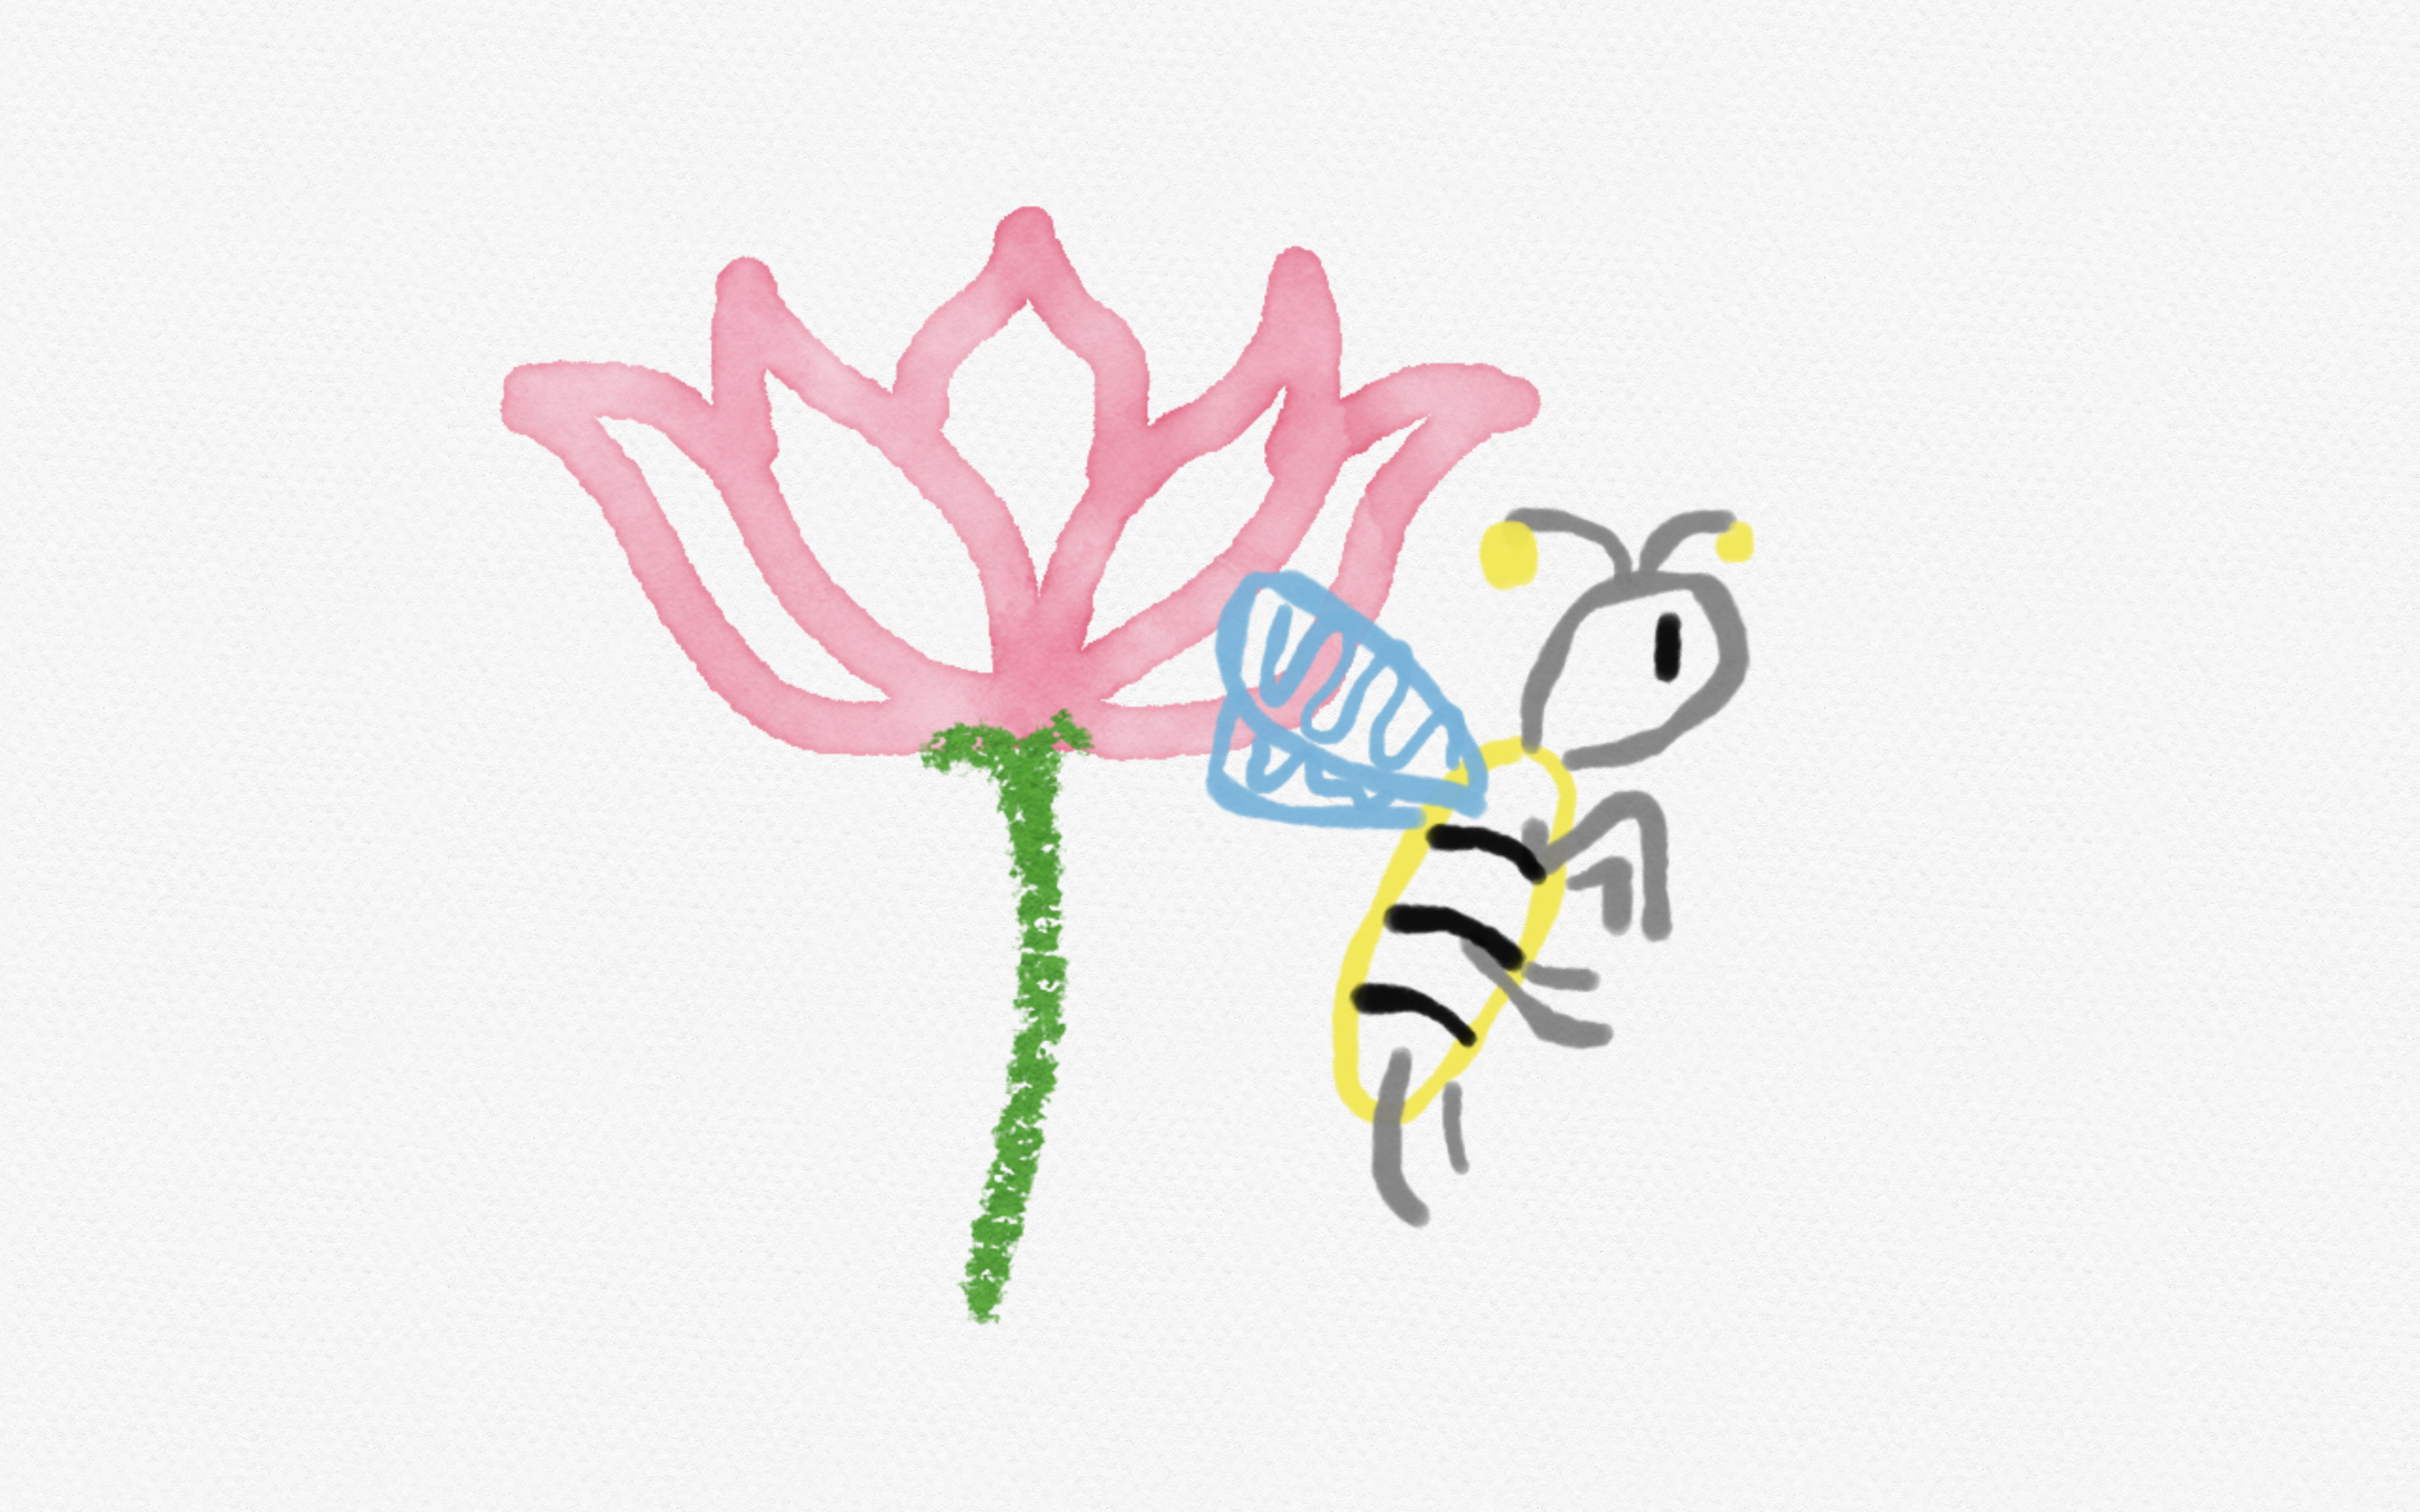
\includegraphics[width = 30em]{Logo}
\end{figure}
\newpage
\tableofcontents
\newpage

%----------------------------------------------------------------------Kapitel 1--------------------------------------------------------------------------------------------

\section{Milestones}

%----------------------------------------------------------------------Kapitel 2--------------------------------------------------------------------------------------------

\section{Arbeitspakete}

%----------------------------------------------------------------------Kapitel 3--------------------------------------------------------------------------------------------

\section{PERT-Diagramm}

%----------------------------------------------------------------------Kapitel 4--------------------------------------------------------------------------------------------

\section{Spezialgebiete}

%----------------------------------------------------------------------Kapitel 5--------------------------------------------------------------------------------------------

\section{Whitebox-Tests}
\sectionauthor{Sergei Pravdin}
Ein Entwickler implementiert nicht nur Arbeitspakete, für die er zuständig ist, sondern auch entsprechende für diese Arbeitspakete Whitebox-Test, um etwaige Bugs sofort in Quell-Code zu korrigieren. Whitebox-Test werden klassisch (nach der Implementierung der Klassen) und ohne TDD geschrieben. Die Arbeitspakete werden durch die Verbindung mit der Datenbank getestet, wenn der Zustand der Anwendung es ermöglicht. Sonst werden fehlende Bestandteile von Mockito oder PowerMock gemockt. Jedes Arbeitspaket hat mindestens einen Testfall. Die Tests werden mit dem Projekt mitgeliefert.

­\subsection{Milestone 1}

\subsubsection{Meta - Logger}
Für den Test des Loggers bekommen wir zuerst getInstance() und rufen die Methode development(''testMessage'') auf. Der Test ist bestanden, wenn das Ergebnis der Methode getMessage() ''testMessage'' ist.

\subsubsection{Meta - ConfigReader}
Um den ConfigReader zu testen, bekommen wir getInstance() und rufen getSystemConfigurations() auf. Als Ergebnis wird ein eine richtige Config-Propertie erwartet. WO IST DAS CONFIG-FILE?

\subsubsection{Utilities I}
Der Test ist für ein ApplicationDao zuständig. Ein ApplicationDto 'testDto' wird erstellt und durch testDto.setName(''testName'') ausgefüllt. Danach wird eine Methode ApplicationDao.createCustomization(testDto) aufgerufen. Der Test ist bestanden, wenn eine Methode ApplicationDao.readCustomization(testDto).getName() ''testName'' ist.

\subsubsection{Utilities II}
Welche Klassen?

\subsubsection{System Start}
Die Methode DataLayerInitializer.setUpConnectionPool() wird aufgerufen. Der Test ist bestanden, wenn ConnectionPool.getInstance() nicht null ist.

\subsubsection{Facelets}
Eine Methode logOut() von einem Footer wird aufgerufen. Der Test ist bestanden, wenn das Ergebnis ''logIn.xhtml?faces-redirect=true'' ist.

\subsubsection{Exception handling}
Wir wollen eine Fehlerseite testen, deshalb wird ErrorDto 'testErrorDto' erzeugt und durch setMessage(''testErrorMessage'') ausgefüllt. Dann wird eine Methode setErrorDto(testErrorDto) aufgerufen. Der Test ist bestanden, wenn das Ergebnis der Methode getMessage von der Klasse 'Error' 'testErrorMessage' ist.

\subsubsection{User Authentication - Registration}
Ein UserDto 'userDto' wird erzeugt. Dann werden eine Methode userDto.setId(1), userDto.setPassword(testPassword) und userDto.setEmailAddress(testSep21email@gmail.com) aufgerufen. Im nächsten Schritt wird die Methode 'register()' in der Klasse 'Registration' aufgerufen. Diese Methode muss eine Interaktion mit einem UserDao, genauer gesagt mit der Methode 'UserDao.createUser(userDto)' implementieren, deshalb ist der Test bestanden, wenn das Ergebnis der Methode 'UserDao.readUserByEmail(userDto).getId()'  ''1'' ist.

\subsubsection{User Authentication - LogIn (erfolglos)}
Eine Methode setEmail(wrongEmail) und eine Methode setPassword(wrongPassword) aus der Klasse Login werden aufgerufen. Im nächsten Schritt wird eine Methode logIn() aufgerufen. Das Ergebnis muss ''null'' sein, damit der Test als bestanden gilt. 

\subsubsection{User Authentication - LogIn (erfolgreich)}
Eine Methode setEmail(testSep21email@gmail.com) und eine Methode setPassword(testPassword) aus der Klasse Login werden aufgerufen. Im nächsten Schritt wird eine Methode logIn() aufgerufen. Das Ergebnis muss ''profile?id=1'' sein, damit der Test als bestanden gilt.

\subsubsection{User Authentication - User Delete}
Ein UserDto 'userDto' wird erzeugt. Dann werden eine Methode userDto.setId(1), userDto.setPassword(testPassword) und userDto.setEmailAddress(testSep21email@gmail.com) aufgerufen. Im nächten Schritt wird eine Methode readUserByEmail(userDto).
Ein erhaltenes UserDto wird wieder durch die Methode UserDao.deleteUser(userDto) übergeben. Der Test ist bestanden, wenn das Ergebnis der Methode UserDao.readUserByEmail(userDto) ''null'' ist. Das bedeutet, dass kein Nutzer mit der ID '1' in der Datenbank existiert.

\subsubsection{Global app management}
Ein ApplicationDto 'testDto' wird erzeugt. Dann wird die Methode setApplication(testDto) aufgerufen. Im nächsten Schritt werden die Methode testDto.setSiteNotice(testNotice) und save() aus der Klasse 'Administration' aufgerufen. Der Test gilt als bestanden, wenn die Methode getApplication().getSiteNotice() aus der Klasse 'SiteNotice' das Ergebnis ''testNotice'' liefert.

­\subsection{Milestone 2}
\subsubsection{User management I - Сhange Password}


\end{document}
